\section{Matrix Factorization Visualization}

For each movie \textit{j} we visualize it as a 2D vector using the coordinates $\bar{V}[1:2,j]$, where $\bar{V}$ is obtained from the previous section. We show 10 random movies in Figure~\ref{fig:tenRandom}, the most popular 10 movies in Figure~\ref{fig:tenMostPopular} and the best 10 movies in Figure~\ref{fig:tenBest}. In general there is little correlation between distance in the plots and movie similarity as seen by the authors. For example, Scream and Star Wars are very close in Figure~\ref{fig:tenMostPopular} but we don't think they are very similar.\\
We observe that the most popular 10 movies are located along the line $(1,1)$ while the best 10 movies cover the 2D space more uniformly. This distribution is still unclear and it might be a coincidence. 
Figure~\ref{fig:tg} shows the representation for the genres horror, children and fantasy. The movies within each genre are loosely cluster together, for example horror movies are mostly located on the bottom left corner and fantasy movies on the upper right corner. We can visualize the mean representation with its variance for each genre in Figure~\ref{fig:tgMV}. In general the variance as large as the distance between mean centers, therefore we should expect loose clusters are observed. 

\begin{figure}[hptb]
\centering
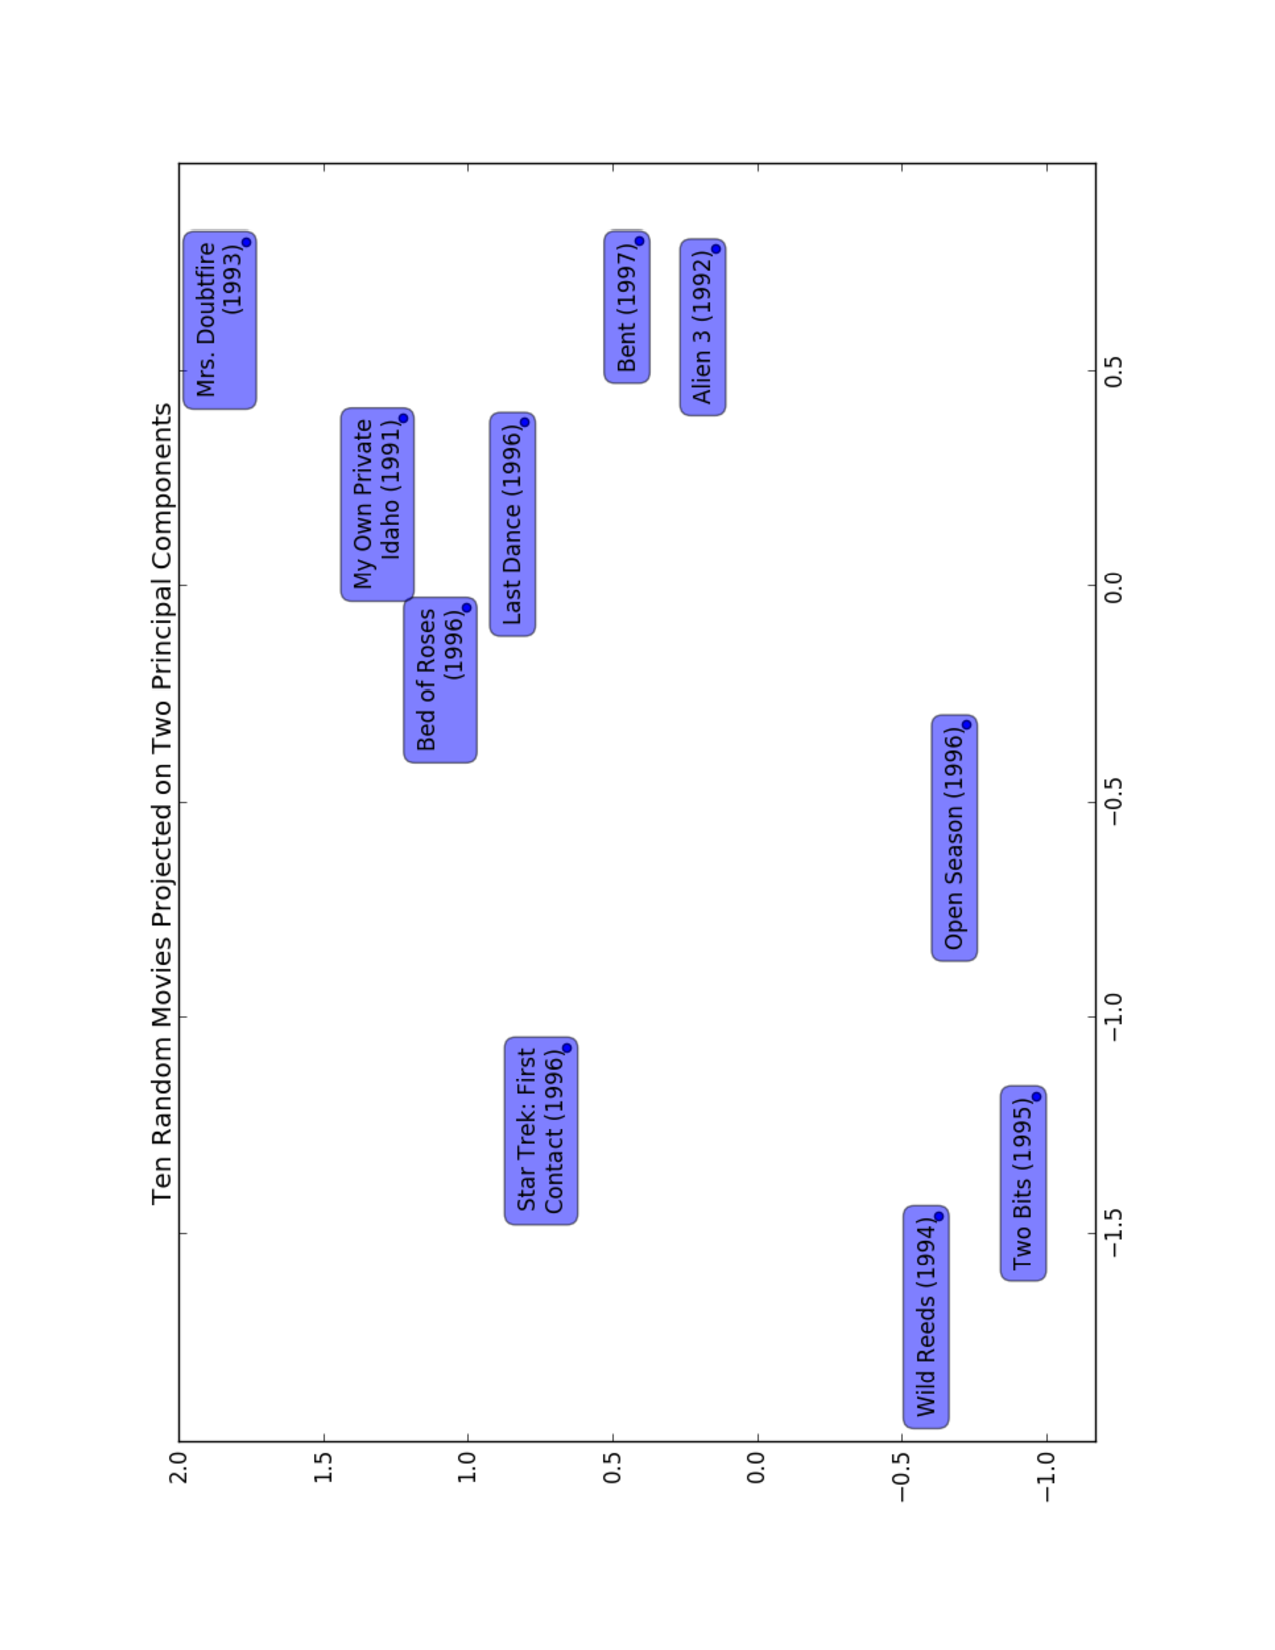
\includegraphics[width=0.8\textwidth, angle =270]{Random_10_Movies.pdf}
 \caption{Ten Random movies projected along two principal components.}
\label{fig:tenRandom}
\end{figure}


\begin{figure}[hptb]
\centering
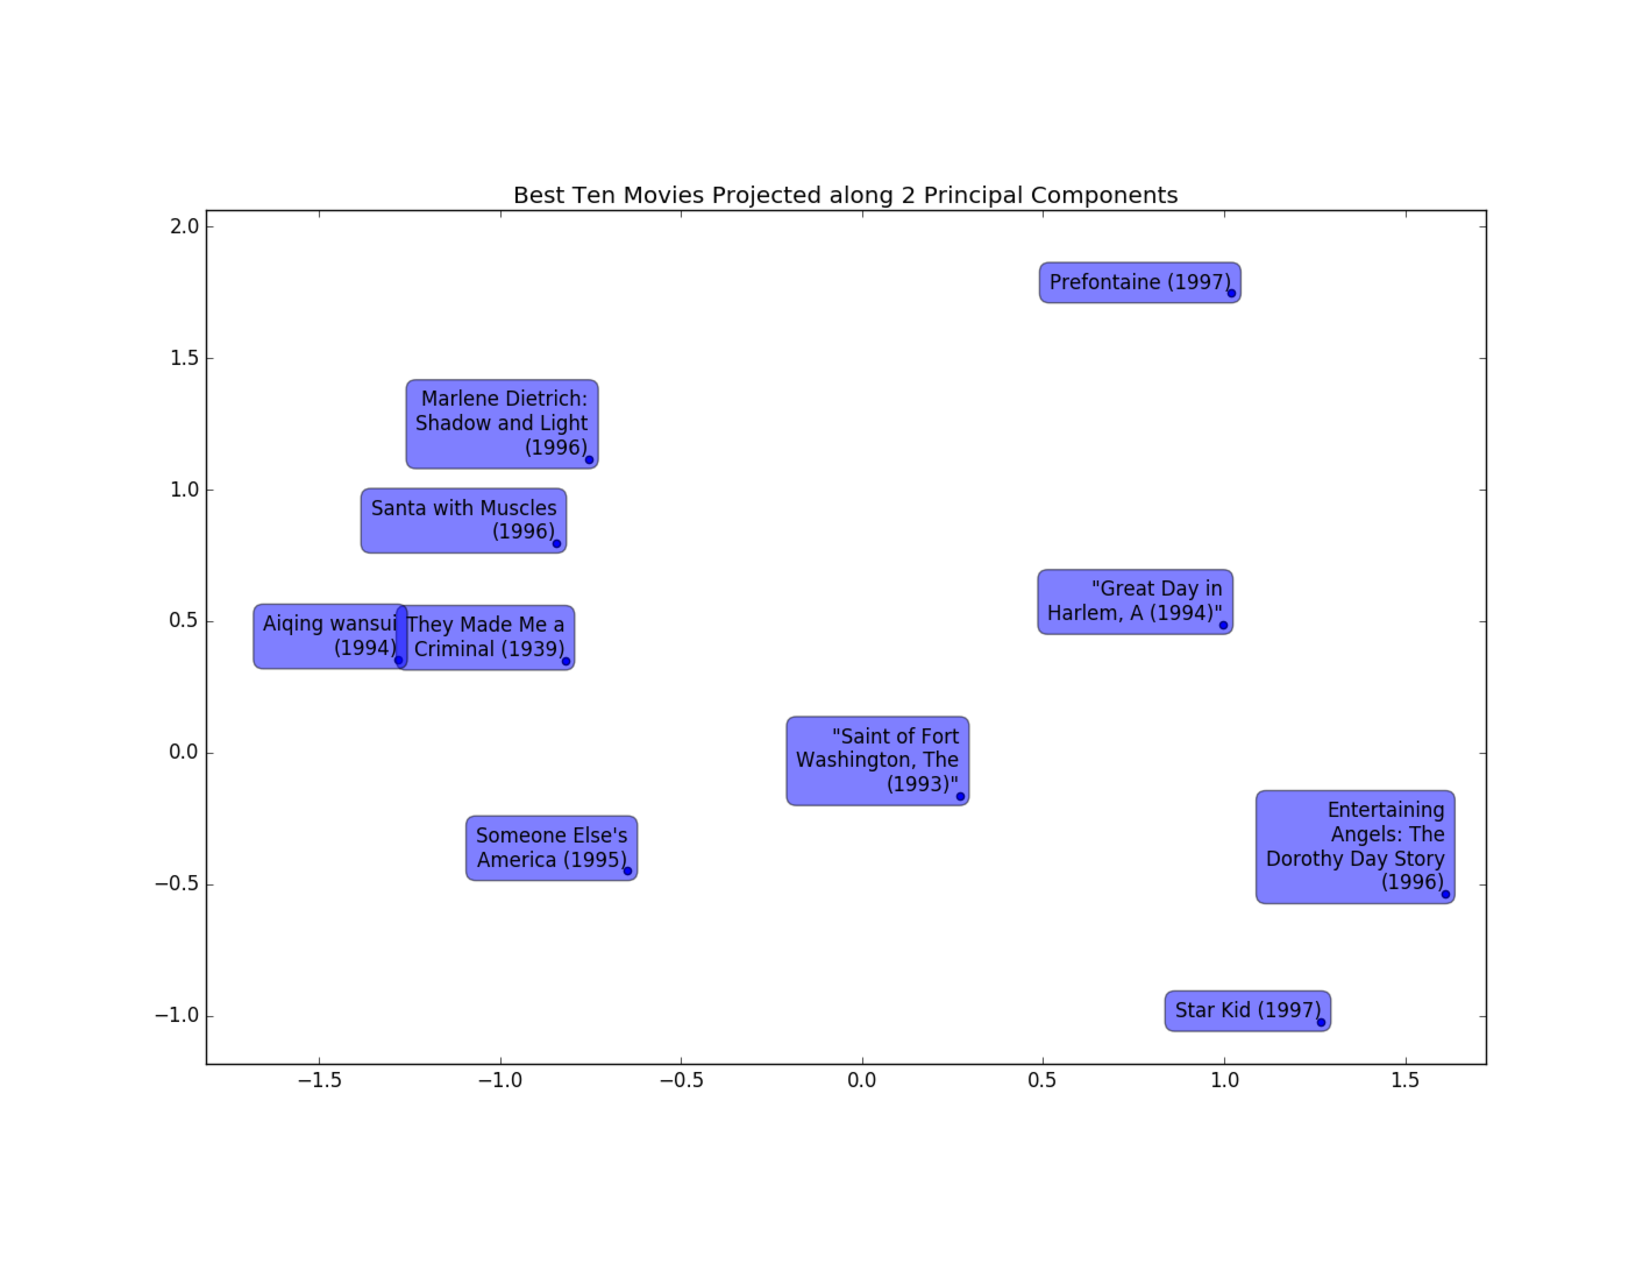
\includegraphics[width=0.8\textwidth, angle = 270]{Best_10_Movies.pdf}
 \caption{Best ten movies projected along two principal components.}
\label{fig:tenBest}
\end{figure}


\begin{figure}[hptb]
\centering
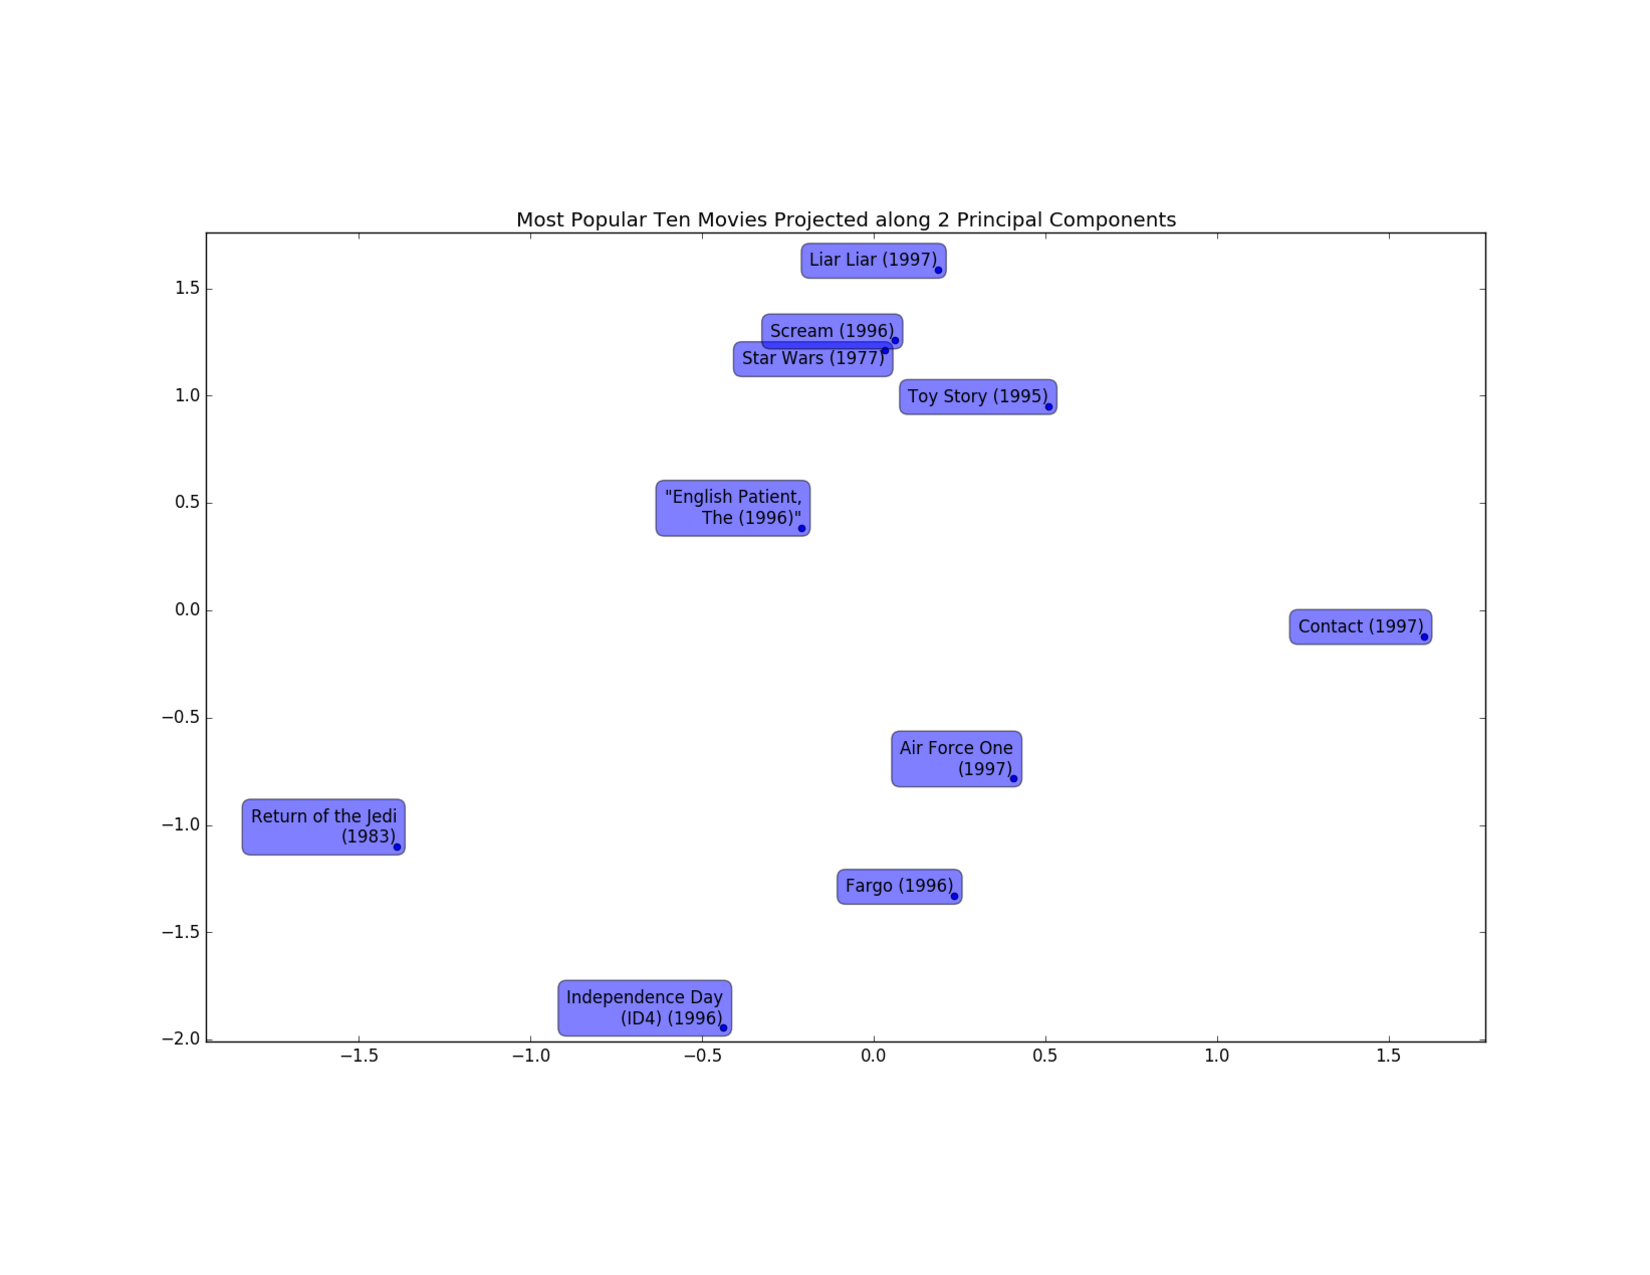
\includegraphics[width=0.8\textwidth, angle =270]{Popular_10_Movies.pdf}
 \caption{Most popular ten movies projected along two principal components.}
\label{fig:tenMostPopular}
\end{figure}


\begin{figure}[hptb]
\centering
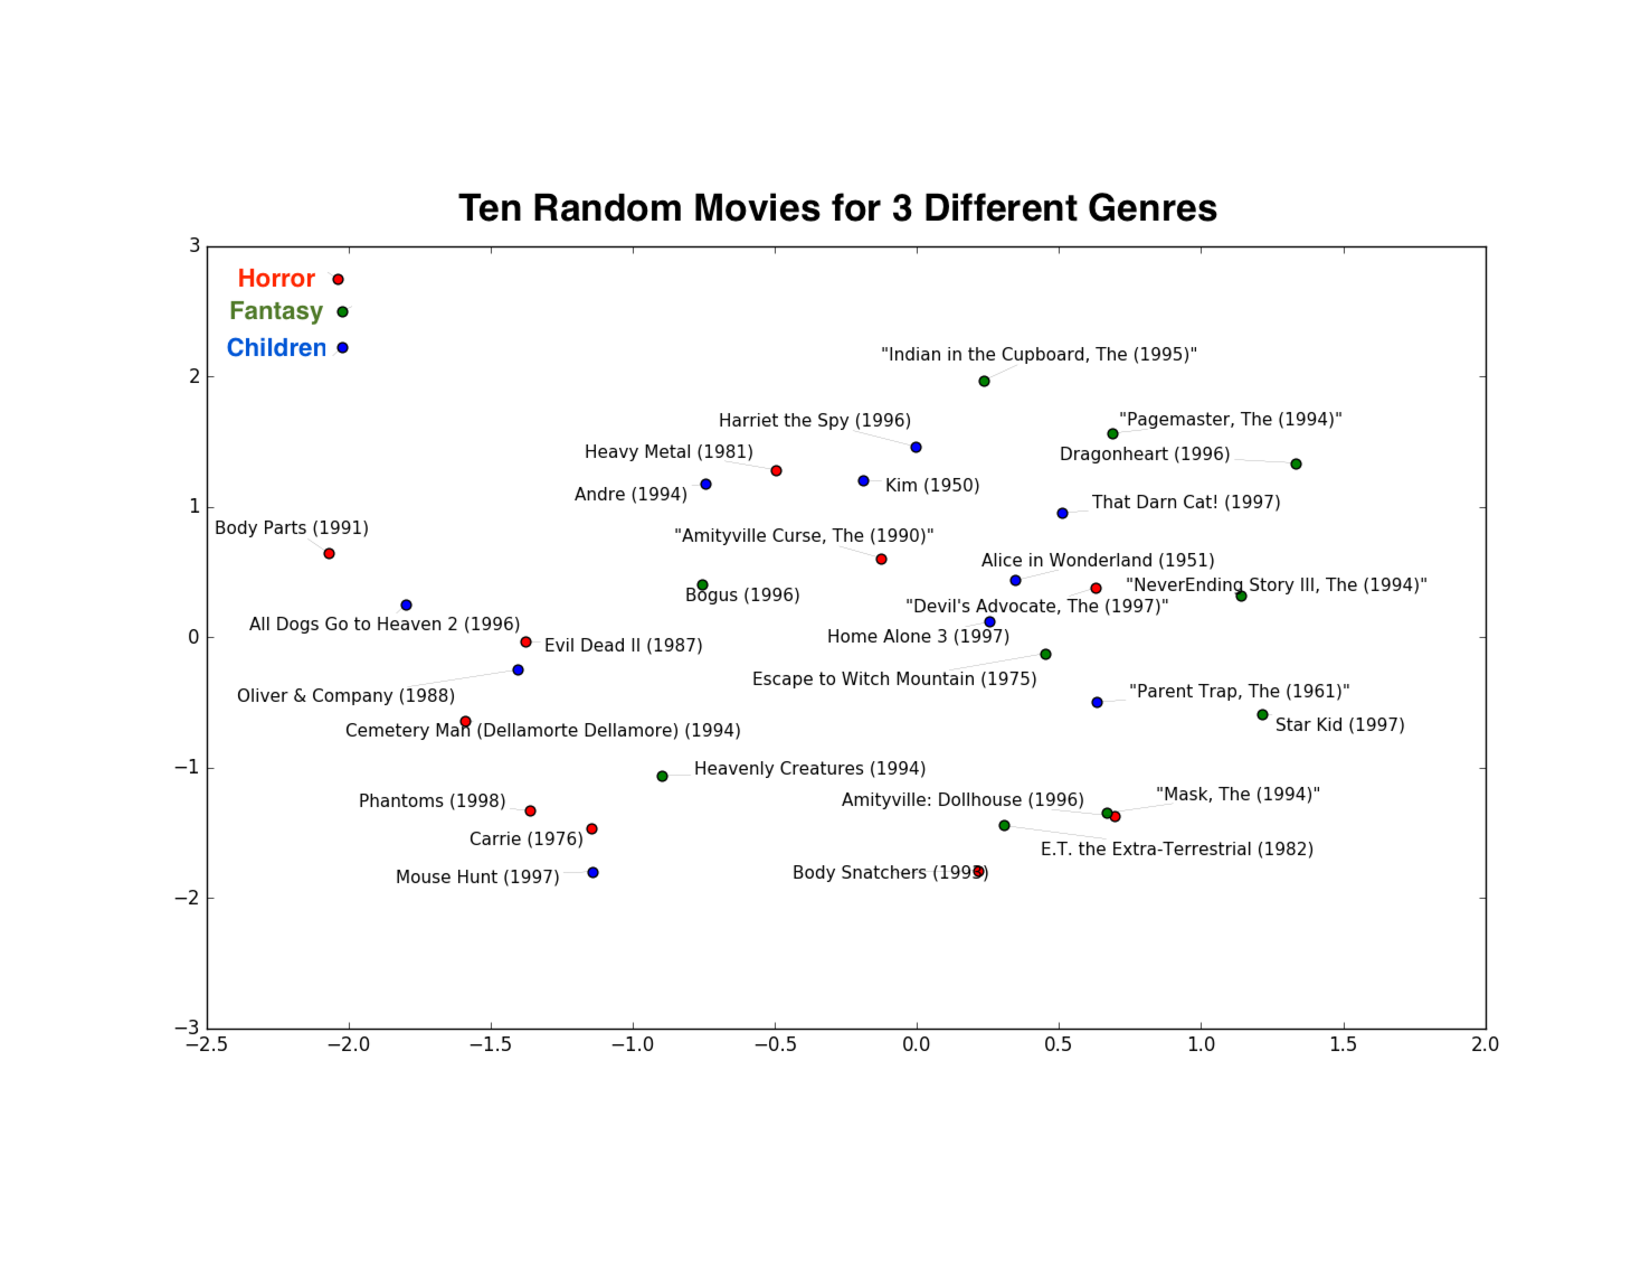
\includegraphics[width=0.8\textwidth, angle =270]{Three_Genres.pdf}
 \caption{Ten random movies for the genres horror, fantasy and children. }
\label{fig:tg}
\end{figure}


\begin{figure}[hptb]
\centering
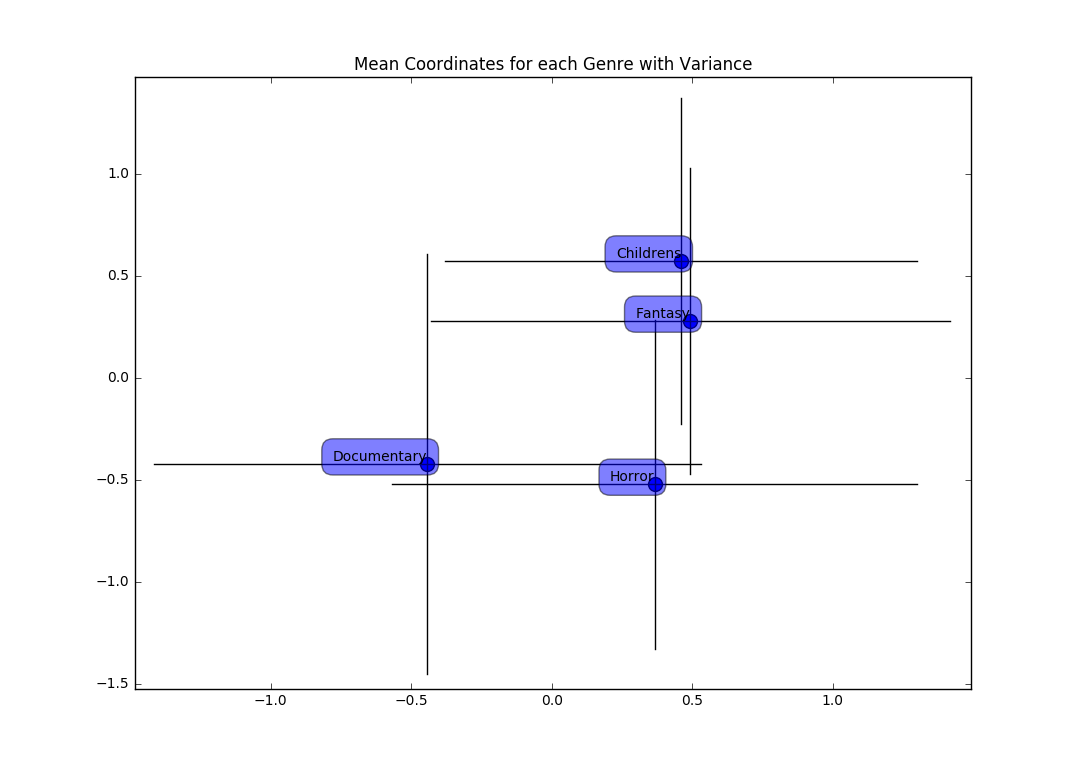
\includegraphics[width=0.8\textwidth, angle =0]{Mean_Genre_Variance.png}
 \caption{Mean Coordinates for each genre with variance. We also show documentary for reference with a genre far from our selection.}
\label{fig:tgMV}
\end{figure}
